\ProvidesFile{ch-background-signals.tex}[Background Model]
\chapter{Background Model}
\graphicspath{{/Users/liamrobinson/Documents/PyLightCurves/docs/build/html/_images}}

Whenever an optical telescope is observing an unresolved space object, the object's signal is necessarily superimposed on whatever signals exist in the background as the unresolved signal spreads much further than the object's actual geometric bounds. In this context, background does not only refer to sources physically further than the object --- as light can easily enter optical path through atmospheric scattering --- but all sources that impact the image apart from the object signal. Some of these sources even originate within the telescope optics and its sensor. To faithfully simulate a telescope observing an object, many position-based SDA tasks are able to ignore background effects while acquiring or tracking objects. For photometry-based SDA, the background is critical. The overall noise floor can be broken up into background signal sources and sensor effects.

\section{Background Signal Sources}

\subsection{Airglow}

Certain chemical reactions from 80-110 km altitude in the upper atmosphere release visible light
\cite{krag2003}. This effect is known as
airglow. Since these reactions are assumed to be isotropic ---  equally intense when integrated along any
vertical line extending upwards from the surface. The airglow signal $\textrm{AINT}$ is modeled in a
similar fashion to integrated starlight. Given the airglow spectra $\textrm{GLINT}(\lambda) \:
\left[ \frac{W}{m^2\cdot m \cdot sr} \right]$, the airglow signal is computed via Eq \ref{eq:aint}.

\begin{equation} \label{eq:aint}
 \textrm{AINT} = \frac{\pi D^2}{4}
  \int_{10^{-8}}^{10^{-6}}{ \textrm{GLINT}(\lambda) \cdot \textrm{QE}(\lambda) \cdot \textrm{ATM}(\lambda)
  \cdot \left( \frac{\lambda}{h c} \right) \: d\lambda}  
\end{equation}

The quantity $\textrm{AINT}$ has units $\left[ \frac{1}{s\cdot sr} \right]$, meaning that the
mean airglow signal in ADU per pixel is simply given by Eq \ref{eq:airglow_adu}

\begin{equation} \label{eq:airglow_adu}
  \bar{S}_{airglow} = AINT \cdot \textrm{AM}(\theta_z) \cdot \Delta t \cdot \left( \frac{\pi s_{pix}}{648000} \right)^2
\end{equation}

In Eq \ref{eq:airglow_adu}, $\textrm{AM}(\theta_z)$ is the relative airmass function which accounts for the accumulation of air along the optical path at different zenith angles \cite{frueh2019notes}. This airmass is termed \textit{relative} as it relates the ratio of absolute airmass at a zenith angle to the absolute airmass at zenith. Often, this function is approximated by the Van-Rhijn factor $\textrm{AM}(\theta_z) = \sec{\theta_z}$ which remains accurate up to $\theta_z \approx 70^\circ$ before diverging to infinity. Instead, a function proposed by Pickering is used \cite{pickering2002}.

\begin{equation} \label{eq:pickering_airmass}
  \textrm{AM}(\theta_z) = \frac{1}{\sin\left((90 - \theta_z) +  \frac{244}{165 + 47 * \left(90 - \theta_z \right)^{1.1}}\right)}
\end{equation}

Using Eq \ref{eq:pickering_airmass} instead of the Van-Rhijn factor is important for computing background signals near the horizon. Figure \ref{fig:airmass_fcns} displays this comparison in action.

\begin{figure}[ht]
  \centering
  \includegraphics[width=\figmed]{sphx_glr_vr_factor_001.png}
  \caption{Airmass function comparison. The Van-Rhijn factor diverges to $+\infty$ while Pickering's function reaches the correct maximum of $\textrm{AM}(\theta_z) \approx 40$.}
  \label{fig:airmass_fcns}
\end{figure}

\begin{figure}[ht]
  \centering
  \includegraphics[width=\figmed]{sphx_glr_background_signals_005.png}
  \caption{Mean airglow signal on the local observer hemisphere. The observer is in New Mexico, USA at
  \pogslla}
  \label{fig:airglowhemi}
\end{figure}

\subsection{Light Pollution}

Another source of background noise light pollution. On a cloudless night with low levels of atmospheric aerosols, 
the zenith surface brightness is approximately $22 \: \left[ \frac{mag}{arcsec^2}
\right]$ (MPSAS) \cite{krag2003}. As light pollution increases, this zenith brightness may dip down to
$14-15 \: \left[ \frac{mag}{arcsec^2} \right]$. To get accurate localized zenith brightness values,
we use the 2015 World Atlas of Sky Brightness dataset \cite{falchi2016_data}. The data is reported in $\left[
	\frac{mcd}{cm^2} \right]$ on a 30-arcsecond grid, requiring conversion to a more useful unit. A subset of the global dataset is displayed in \ref{fig:pollution_data} This conversion is listed in Eq \ref{eq:cd_per_m2_to_mpsas}, using a monochromatic $\lambda = 474$ nm to fit Falchi et al.'s example conversions \cite{falchi2016}.  

\begin{figure}[ht]
  \centering
  \includegraphics[width=\figmed]{sphx_glr_nightlights_001_2_00x.png}
  \caption{Zenith light pollution in the eastern USA, data from \cite{falchi2016_data}}
  \label{fig:pollution_data}
\end{figure}

The mean light pollution CCD signal in ADU per pixel is formulated similarly to airglow. The station's zenith surface brightness $B_{poll,z}$ in MPSAS, linearly interpolated from the World Atlas dataset, is converted to irradiance per steradian via \ref{eq:mpsas_to_irrad_per_ster} and to ADU per pixel via \ref{eq:pollution_adu}. Note that Krag does not implement a specific light pollution model, but instead takes the dark sky site zenith brightness of $22$ MPSAS as input to an atmospherically scattered light model. This is simply an adaptation of Krag's model with a variable zenith brightness.
 
\begin{equation} \label{eq:pollution_adu}
  \bar{S}_{pollution} = B_{poll,z} \cdot SINT \cdot \textrm{AM}(\theta_z) \cdot \Delta t \cdot \left( \frac{\pi s_{pix}}{648000} \right)^2
\end{equation}

\begin{figure}[ht]
  \centering
  \includegraphics[width=\figmed]{sphx_glr_background_signals_003.png}
  \caption{Mean light pollution signal on the local observer hemisphere. The observer is in New Mexico, USA at
  \pogslla}
  \label{fig:pollution_hemi}
\end{figure}

\subsection{Twilight}

Even after the Sun sets, scattered sunlight in the upper atmosphere creates a signal on our CCD. The twilight model implemented for this work is due to Patat et al. and was developed for the European Southern Observatory at Paranal in Chile \cite{patat2006}. This model implements the zenith brightness as a function of the solar zenith angle $\gamma$ --- the angle from zenith to the Sun's apparent centroid. Patat et al.'s model fits a second-degree polynomial in $\gamma$ to approximately 2000 observations in varying atmospheric conditions, yielding separate curves for each of the UBVRI passbands. For example, for the V band, the twilight zenith brightness in MPSAS is given by \ref{eq:b_zenith_twilight} \cite{patat2006}.

\begin{equation} \label{eq:b_zenith_twilight}
  B_{twi,z} = 11.84 + 1.518(\gamma - 95^\circ) - 0.057 (\gamma -  95^\circ)^2
\end{equation}

Eq \ref{eq:b_zenith_twilight} is valid from $95^\circ \leq \gamma \leq 105^\circ$. While $\gamma \le 95^\circ$, the zenith brightness is taken to be constant and equal to the brightness at $\gamma = 95^\circ$. This is not accurate, as it predicts daylight to be the brightness of twilight, but is sufficiently bright to correctly forbid daytime observations by lowering the SNR drastically. After $\gamma = 105^\circ$ the zenith surface brightness is set to $B_{twi,z} = 22$ MPSAS to match the optimal observation condition of the light pollution model \cite{krag2003}. Zenith twilight brightness is plotted as a function of $\gamma$ in Figure \ref{fig:twilight_model}.

\begin{figure}[ht]
  \centering
  \includegraphics[width=\figmed]{sphx_glr_twilight_model_001_2_00x.png}
  \caption{Twilight model surface brightness at zenith as a function of solar zenith angle}
  \label{fig:twilight_model}
\end{figure}

Computing the mean CCD signal in ADU per pixel due to the twilight brightness proceeds identically to the light pollution formulation. 

\begin{equation} \label{eq:twilight_adu}
  \bar{S}_{twilight} = B_{twi,z} \cdot SINT \cdot \textrm{AM}(\theta_z) \cdot \Delta t \cdot \left( \frac{\pi s_{pix}}{648000} \right)^2
\end{equation}

\begin{figure}[ht]
  \centering
  \includegraphics[width=\figmed]{sphx_glr_background_signals_006.png}
  \caption{Mean twilight signal on the local observer hemisphere. The observer is in New Mexico, USA at
  \pogslla}
  \label{fig:pollution_hemi}
\end{figure}

\subsection{Integrated Starlight}

Stars are almost always present in optical images of space objects. The brightest stars streaking across the field of view in Figure \ref{fig:pogs_observation_example} have high SNRs and stand out clearly against the dark background. This raises a question: if the telescope observes a full $1^\circ \times 1^\circ$ area of the sky, where are the rest of the stars? The Milky Way alone contains approximately $1\cdot10^{11}$ stars. The answer is clear: many more stars are present in the image, most of them falling into the background. This residual faint starlight is called "integrated" starlight. 

\begin{figure}[ht]
  \centering
  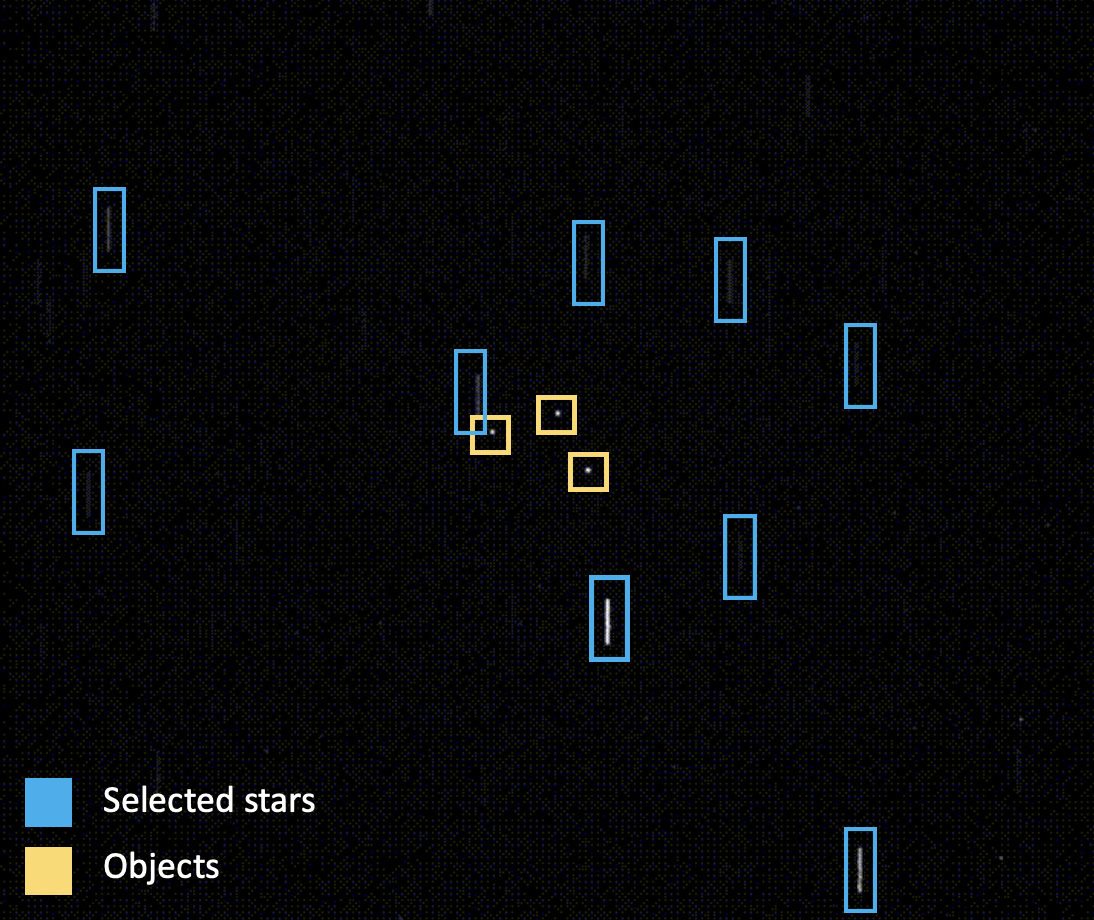
\includegraphics[width=\figmed]{static_images/static_pogs_annotated.png}
  \caption{Raw image of three GEO objects with stars streaking through the background. As expected the star signals have a variety of signal-to-noise ratios. Taken by the Purdue Optical Ground station at \pogslla by Nathan Houtz.}
  \label{fig:pogs_observation_example}
\end{figure}

Krag \cite{krag2003} modeled this signal by building a $1^\circ \times 1^\circ$ grid of surface
brightness values for the full inertial sphere, parameterized by RA/Dec. Krag used the
Guide Star catalog, which contains 15 million stars down to apparent magnitude 16. Exponential extrapolation
was used to predict star counts in each bin for higher magnitudes \cite{krag2003}. Twenty years later, larger star catalogs exist that are nearly complete to much higher apparent magnitudes. The integrated
starlight catalog used in this work was built from the GAIA catalog with approximately 1.5 billion
stars down to magnitude 21-22 \cite{gaia_dr3}. The same $1^\circ \times 1^\circ$ grid was computed
using the \texttt{astroquery.gaia} Python package \cite{astroquery_gaia}. Figure
\ref{fig:gaiapatched} shows the computed brightness map, in units of $S_{10}$. 

\begin{figure}[ht]
  \centering
  \includegraphics[width=\figbig]{sphx_glr_gaia_patched_catalog_001_2_00x.png}
  \caption{Integrated starlight brightness map}
  \label{fig:gaiapatched}
\end{figure}

With this map of exoatmospheric mean brightness of the night sky due to integrated
starlight, the corresponding signal mean in the telescope CCD is computed, adopting Krag's formulation \cite{krag2003}.

\begin{equation} \label{eq:bint}
 \textrm{BINT} = \frac{\pi D^2}{4}
  \int_{10^{-8}}^{10^{-6}}{ \textrm{STRINT}(\lambda) \cdot \textrm{QE}(\lambda) \cdot \textrm{ATM}(\lambda)
  \cdot \left( \frac{\lambda}{h c} \right) \: d\lambda}  
\end{equation}

In Eq \ref{eq:bint}, $D$ is the telescope aperture diameter in meters, $h$ is Plank's constant in
$\left[ \frac{m^2 kg}{s} \right]$, and $c$
is the speed of light in vacuum in $\left[ \frac{m}{s} \right]$. The resulting quantity
$\textrm{BINT}$ has units of $\left[ \frac{1}{s} \right]$, representing the mean total photons passing
through the telescope aperture due to integrated starlight. 

\begin{equation} \label{eq:starlightmean}
  \bar{S}_{star} = 10^{-4} \cdot BINT \cdot \left( \frac{s_{pix}}{3600} \right)^2 \cdot \Delta t \cdot
  b_{is}
\end{equation}

In Eq \ref{eq:starlightmean}, $b_{is}$ is the integrated starlight brightness in $\left[ S_{10}
\right]$ computed by linearly interpolating the dataset in Figure \ref{fig:gaia_patched}, $s_{pix}$ is the telescope pixel scale in $\left[ \frac{arcsecond}{pix} \right]$, and $\Delta t$ is the integration time in seconds. Note the addition of the $10^{-4}$ factor to reconcile catalog surface brightness in terms of 10th magnitude stars, and the 0th magnitude source in $\textrm{BINT}$. This yields $\bar{S}_{star}$ with units $\left[ \frac{e^-}{pix^2} \right]$; photoelectron counts (ADU) per pixel. Figure \ref{fig:starlight_hemi} shows the background signal mean due to integrated starlight.

\begin{figure}[ht]
  \centering
  \includegraphics[width=\figmed]{sphx_glr_background_signals_002.png}
  \caption{Integrated starlight signal on the local observer hemisphere. The observer is in New Mexico, USA at
  \pogslla}
  \label{fig:starlight_hemi}
\end{figure}

\subsection{Scattered Moonlight}

Moonlight scattering through the atmosphere significant increases background brightness \cite{krag2003}. This scattering effect can be decomposed into Rayleigh (isotropically distributed) and Mie (exponentially distributed) scattering modes. The Rayleigh scattered component is computed with Table 4 published by Daniels parameterized by the angle from the observation to zenith $z_{obs}$, the angle from the Moon to zenith $z_{moon}$, and the angle between the observation and the Moon on the horizon $\Delta Az$ \cite{daniels1977}. Interpolating this table yields the intensity of the Rayleigh scattering $F_{rs}$ in $10^{-10}$ $W/(cm^2 \cdot \mu m \cdot sr)$ \cite{krag2003}. The Mie scattered component is formulated with Eq \ref{eq:mie_scattering_moon}.

\begin{equation} \label{eq:mie_scattering_moon}
  F_{ms}(\lambda) = a_1 \left[ e^{-\left(\frac{\Psi}{\Psi_1}\right)} + a_2 e^{-\left(\frac{\pi - \Psi}{\Psi_2}\right)} \right] F_{rs}(\lambda)
\end{equation}

Daniels recommends $a_1 \in [50, 100]$, $a_2 \in [0.01, 0.02]$, $\Psi_1 \in [10^\circ, 20^\circ]$, and $\Psi_2 \approx 50$ \cite{daniels1977}. Prior to any station-specific fitting, the middle of these intervals are chosen, yielding $a_1 = 75$, $a_2 = 0.015$, $\Psi_1 = 15^\circ$, and $\Psi_2 = 50^\circ$. $a_1$ and $a_2$ are dimensionless, such that $F_{ms}$ also has units of $10^{-10}$ $W/(cm^2 \cdot \mu m \cdot sr)$. The total intensity of the scattered moonlight $F_{mt}$ via Eq \ref{eq:total_scattered_moonlight} following Krag's formulation \cite{krag2003}.

\begin{equation} \label{eq:total_scattered_moonlight}
  F_{mt} = f(\theta) \left[ F_{rs}(\lambda) + F_{ms}(\lambda) \right]
\end{equation}

in Eq \ref{eq:total_scattered_moonlight}, $f(\theta)$ is the lunar phase function which describes the fraction of the full Moon brightness is reflected at an observer when the Sun-Moon-observer angle is $\theta$. This function is linearly interpolated within Table 3 in \cite{daniels1977}. Finally, Krag introduces a correction factor $f_{corr}$ to account for the difference between the Sun's irradiance spectrum and the spectrum of scattered moonlight, defined in Eq \ref{eq:krag_f_corr}.

\begin{equation} \label{eq:krag_f_corr}
  f_{corr} = \frac{I_0}{SUN(550 \: \left[\textrm{nm}\right])}
\end{equation}

With all these pieces, the mean scattered moonlight signal in ADU per pixel is computed in Eq \ref{eq:moonlight_adu}.

\begin{equation} \label{eq:moonlight_adu}
  \bar{S}_{moon} = F_{mt}(550 \: \left[\textrm{nm}\right]) \cdot SINT \cdot \left( \frac{s_{pix}}{3600} \right)^2 \cdot \Delta t \cdot f_{corr}
\end{equation}

\begin{figure}[ht]
  \centering
  \includegraphics[width=\figmed]{sphx_glr_background_signals_001.png}
  \caption{Mean scattered moonlight signal on the local observer hemisphere. The observer is in New Mexico, USA at
  \pogslla}
  \label{fig:moonlight_hemi}
\end{figure}

\subsection{Zodiacal Light}

Zodiacal light is an effect created by sunlight reflecting off of dust in the ecliptic plane \cite{krag2003}. Zodiacal light is strongest around the Sun --- an exclusion zone for most optical telescopes --- but also reaches a peak directly away from the Sun due to the opposition effect. This peak is known as the Gegenschein, meaning "opposing light". The zodiacal light brightness is linearly interpolated within Table 1 of \cite{roach1972} which is listed for convenience in Appendix \ref{data:roach_zod}. This reports the surface brightness of the zodiacal light in $S_{10}$, which is used without conversion to find the mean CCD signal in ADU per pixel via Eq \ref{eq:zodiacal_adu}.

\begin{equation} \label{eq:zodiacal_adu}
  \bar{S}_{zod} = BINT \cdot \left( \frac{s_{pix}}{3600} \right)^2 \cdot \Delta t \cdot ZOD \cdot 10^{-4}
\end{equation}

As in the integrated starlight signal, the $10^{-4}$ factor reconciles the $S_{10}$ surface brightness with the 0th magnitude source in $\textrm{BINT}$. 

\begin{figure}[ht]
  \centering
  \includegraphics[width=\figmed]{sphx_glr_background_signals_004.png}
  \caption{Mean zodiacal light signal on the local observer hemisphere. The observer is in New Mexico, USA at
  \pogslla}
  \label{fig:zod_hemi}
\end{figure}

\subsection{Sampling The Background}

Each background signal is only defined in terms of its mean. On a pixel-by-pixel basis, the signal for an exposure is sampled from a Poisson distribution for each background term. This distribution models the number of independent and identically distributed events that occur during a time period. For CCD astronomy, this translates to the event of a photon hitting the sensor. A Poisson distribution is defined on the positive integers by a single parameter $\lambda$ which is both the mean and variance of the distribution. The probability density function (PDF) for the Poisson distribution takes the form of Eq \ref{eq:poisson_pdf} \cite{frueh2019notes}.

\begin{equation} \label{eq:poisson_pdf}
  P_\lambda(x=k) = \frac{\lambda^k e^{-\lambda}}{k!}
\end{equation}

This distribution has a useful property that $P_{\lambda_1 + \lambda_2}(x=k) = P_{\lambda_1}(x=k) + P_{\lambda_2}(x=k)$ so long as the distributions described by $\lambda_1$ and $\lambda_2$ are independent. Our background sources are reasonably assumed to be independent as they each originate from distinct physical processes.

\begin{equation} \label{eq:background_poisson}
  \lambda_{background} = \bar{S}_{airglow} + \bar{S}_{pollution} + \bar{S}_{twilight} + \bar{S}_{star} + \bar{S}_{moon} + \bar{S}_{zod}
\end{equation}

Drawing samples from the Poisson distribution defined by $\lambda_{background}$ computes the background of the CCD image. 

\subsection{Background Source Importance}

Some background signals are more impactful than others. Table \ref{tb:signal_importance} details the approximate magnitudes in photoelectrons per pixel one can expect from a telescope similar to the Purdue Optical Ground Station.

\begin{table}[]
  \begin{tabular}{|l|l|}
  \hline
  \textbf{Source} & \textbf{Magnitude} $\mathbf{\left[ e^- / \textbf{pix}\right]}$ \\ \hline
  Airglow                & $10^3 - 10^4$                              \\ \hline
  Scattered moonlight    & $0 - 10^5$                                 \\ \hline
  Integrated starlight   & $10^1 - 10^2$                              \\ \hline
  Light pollution        & $10^2 - 10^3$                              \\ \hline
  Zodiacal light         & $10^2 - 10^4$                              \\ \hline
  Twilight               & $10^1 - 10^7$                              \\ \hline
  \end{tabular}
  \caption{Background signal importance}
  \label{tb:signal_importance}
\end{table}

\section{Sensor Effects}

\subsection{Dark Noise}

TODO

\subsection{Readout Noise}

TODO

\section{Signal to Noise Ratio (SNR)}

TODO

\section{Sampling Noisy Light Curves}

TODO